\begin{figure}
\centering
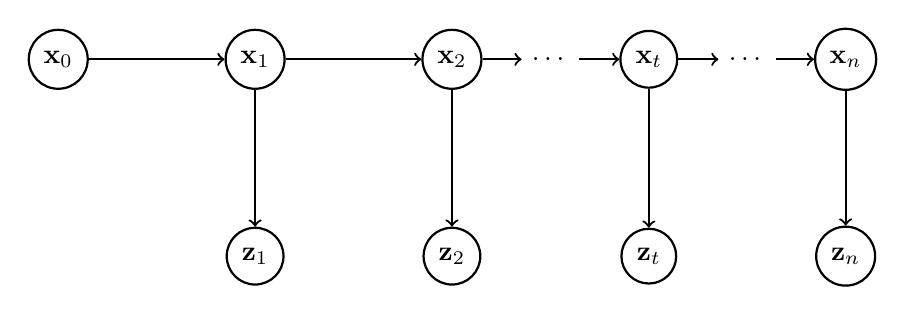
\begin{tikzpicture}
\begin{scope}[every node/.style={circle,thick,draw}]
	\node (x0) at (-2.5,0) {$\mathbf{x}_{0}$};

    \node (x1) at (0,0) {$\mathbf{x}_{1}$};
    \node (z1) at (0, -2.5) {$\mathbf{z}_{1}$};
    
    \node (x2) at (2.5, 0) {$\mathbf{x}_{2}$};
    \node (z2) at (2.5,-2.5) {$\mathbf{z}_{2}$};
    
    \node (xi) at (5, 0) {$\mathbf{x}_{t}$};
    \node (zi) at (5, -2.5) {$\mathbf{z}_{t}$};
    
    \node (xn) at (7.5, 0) {$\mathbf{x}_{n}$};
    \node (zn) at (7.5, -2.5) {$\mathbf{z}_{n}$};
\end{scope}

\begin{scope}[style={thick,draw}]
    \node (xdot1) at (3.75,0) {\dots};
    \node (xdot2) at (6.25,0) {\dots};
\end{scope}


\begin{scope}[style={thick,draw}]
	\path [->] (x0) edge node {} (x1);

    \path [->] (x1) edge node {} (z1);
    \path [->] (x1) edge node {} (x2);
    
    \path [->] (x2) edge node {} (z2);
    \path [->] (x2) edge node {} (xdot1);
    
    \path [->] (xi) edge node {} (zi);
    \path [->] (xdot1) edge node {} (xi);
    \path [->] (xi) edge node {} (xdot2);
    
    \path [->] (xn) edge node {} (zn);
    \path [->] (xdot2) edge node {} (xn);
\end{scope}

\end{tikzpicture}

\caption[A Bayes Net for a Kalman Filter.]{A Bayes Net for a Kalman filter. For brevity's sake, the control vector, $\pmb{u}_{t}$ has been omitted  as it is deterministic and known in each state.}
\label{figure:bayes_net}
\end{figure}